%  !TeX  root  =  user_guide.tex

\section{Plugin Analisi geomorfologica}\label{sec:rasterrain}

% when the revision of a section has been finalized, 
% comment out the following line:
% \updatedisclaimer

Il plugin Analisi geomorfologica (Raster Terrain Modelling) consente di calcolare la pendenza, l'esposizione, 
l'indice di asperità e la curvatura totale da un DEM (Digital Elevation Model). 
È semplice da usare grazie ad un'interfaccia grafica intuitiva: i risultati dell'analisi sono salvati in 
un nuovo layer raster (Figura \ref{fig:raster_terrain_dialog}).
Il plugin richiede che i seguenti parametri siano specificati prima di eseguire l'analisi:

\begin{itemize}[label=--]
\item \textbf{Analisi}: pendenza, esposizione, indice di asperità e curvatura totale
\item \textbf{Layer in input}: selezionare il layer per l'analisi tra i raster caricati in QGIS 
\item \textbf{Layer in output}: specificare nome e percorso del file raster contenente i risultati dell'analisi.
\item \textbf{Formato in output}: specificare il formato del raster dei risultati (GeoTiff è il formato predefinito).
\end{itemize}

Descrizione dell'analisi:

\begin{itemize}[label=--]
\item \textbf{Pendenza}: calcola l'angolo di pendenza per ogni cella espresso in gradi.
\item \textbf{Esposizione}: 0 gradi per nord e continuando in senso orario.
\item \textbf{Indice di asperità}: una misura quantitativa dell'eterogeneità del terreno.
\item \textbf{Curvatura totale}: una misura della curvatura che combina la curvatura piana e di profilo.
\end{itemize}

\begin{figure}[ht]
   \centering
   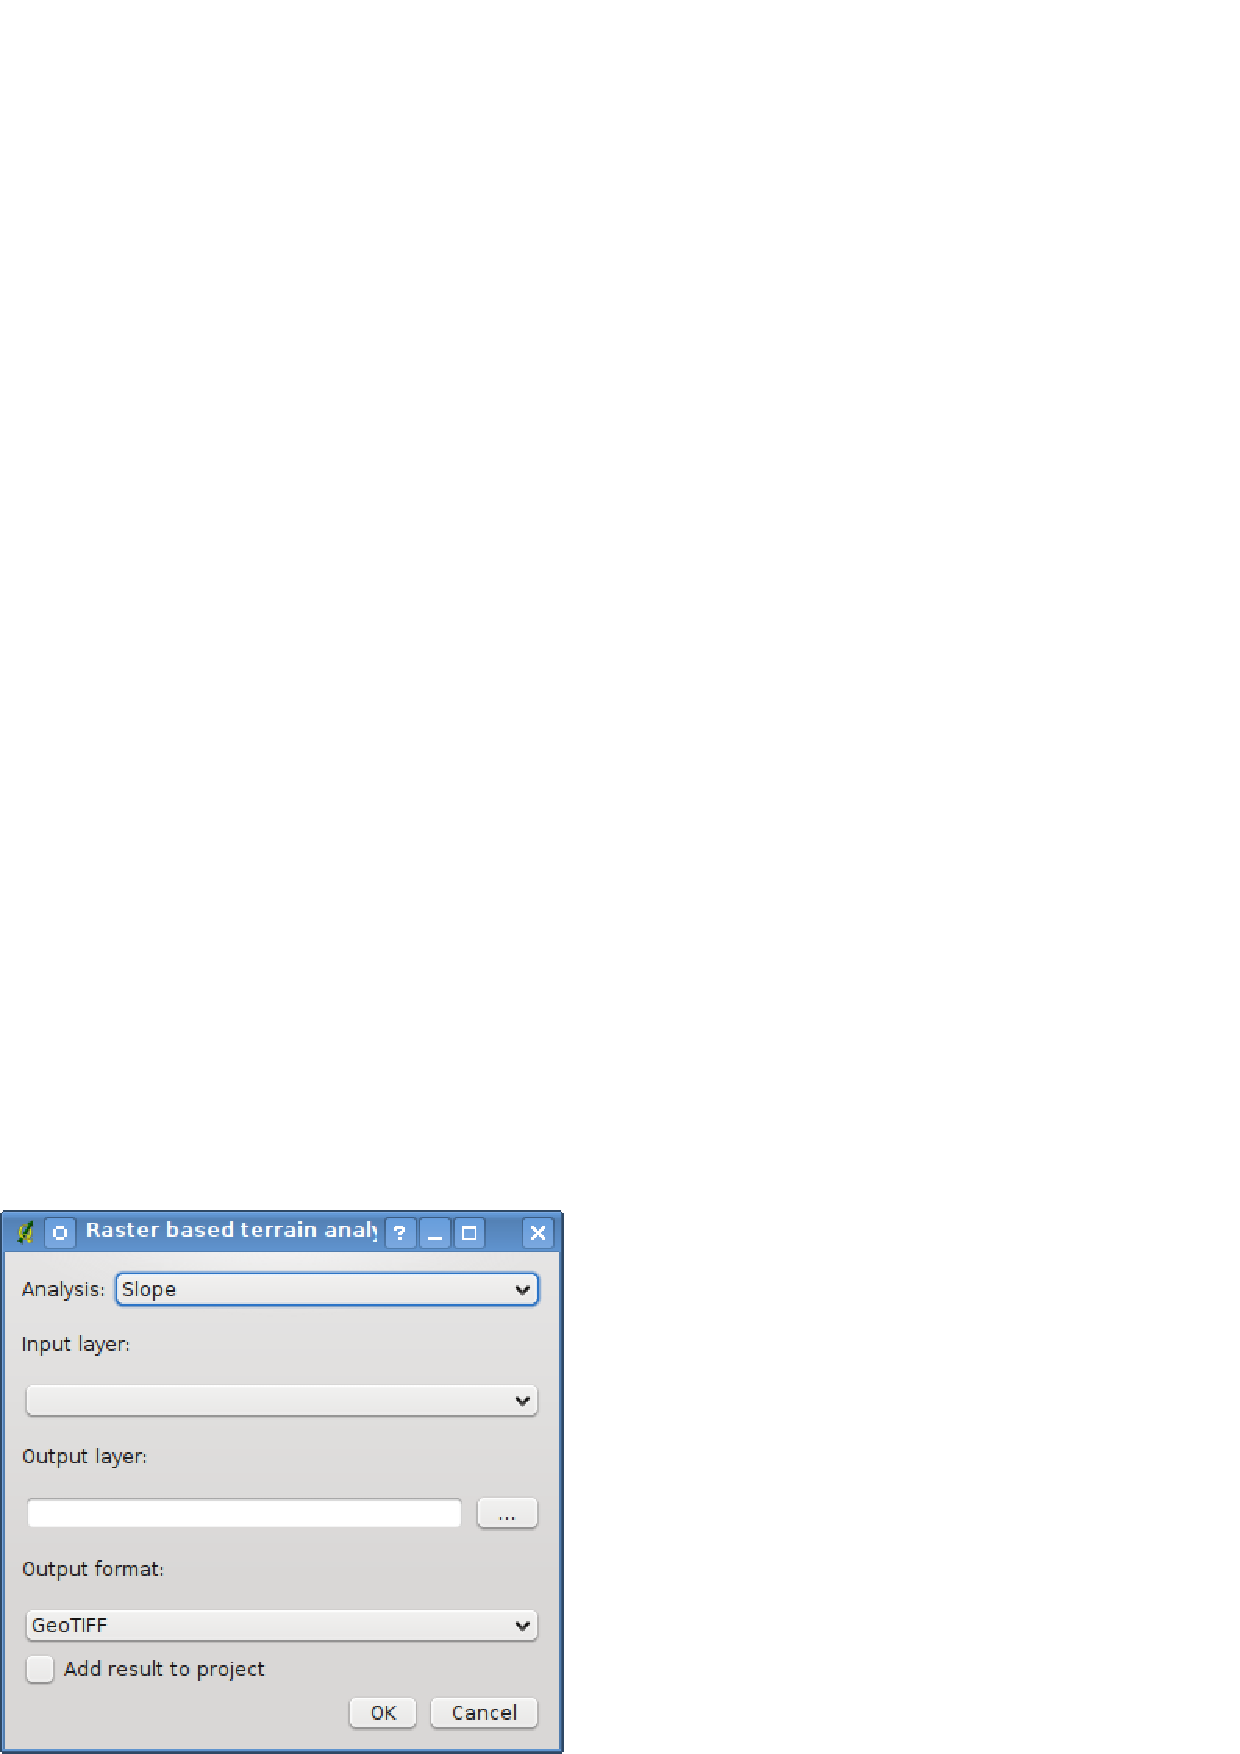
\includegraphics[clip=true, width=9cm]{raster_terrain_dialog}
   \caption{Plugin Analisi geomorfologica \nixcaption}\label{fig:raster_terrain_dialog}
\end{figure}

\minisec{Usare il plugin}\label{raster_terrain_usage}

\begin{enumerate}
  \item Avviare QGIS e caricare un DEM. 
  \item Caricare il plugin dal gestore dei plugin (Sezione \ref{sec:load_core_plugin}) 
  e cliccare sull'icona \toolbtntwo{raster_terrain}{Analisi geomorfologica} nella barra dei plugin. 
 Si aprirà la finestra di dialogo Analisi geomorfologica mostrata in Figura \ref{fig:raster_terrain_dialog}.
  \item Selezionare un metodo di analisi (es. \dropmenuopt{Pendenza}).
  \item Specificare nome, percorso e formato del file di output.
  \item Cliccare su \button{Ok}.
\end{enumerate}

\FloatBarrier
